\documentclass[addpoints,12pt]{exam}
\usepackage{graphicx}
\usepackage{subcaption}
\usepackage{array}
\usepackage{booktabs}
\usepackage{fontspec}
\usepackage{enumitem}
\usepackage{float}
\usepackage{listings}
\usepackage{mdframed}
\usepackage[round]{natbib}
\usepackage{wrapfig}

\begin{filecontents}{ajexam1.bib}
@MastersThesis{CZ,
author = {Cathy Zhang},
title = {A Suit of Case Studies in Relational Database Design},
school = {Department of Computer Science, School of Graduate Studies},
year = {2012}
}
@Book{GTM,
author = {Goodrich, Michael T and Tamassia, R and Mount, David M},
title = {Data Structures and Algorithms in C++},
publisher = {John Wiley \& Sons},
year = {2003}
}

\end{filecontents}

\begin{document}
\pointsinrightmargin
\bracketedpoints
\pagestyle{headandfoot}
\runningheadrule
\firstpageheader{}{}{}
\runningheader{Midterm Exam\\}{CSE4047.1: Advanced Java\\Course Teacher: [KMH] Monirul Hasan}{Summer 2018\\July 16, 2018}
\firstpagefooter{}{Page \thepage\ of \numpages}{}
\runningfooter{}{Page \thepage\ of \numpages}{}

\begin{center}
\begin{tabular}{|ll|ll|}
%\hline
\multicolumn{4}{c}{\Large{\textbf{\setmainfont{Agency FB}SOUTHEAST UNIVERSITY}}}\\
\multicolumn{4}{c}{Department of CSE, SSE}\\
\multicolumn{4}{c}{Summer 2018 Midterm Exam}\\
\multicolumn{4}{c}{}\\
\hline
\textbf{Program}		&	B. Sc. in CSE		&	\textbf{Section}	&	1 (KMH)\\
\textbf{Course Code}	&	CSE2021				&	\textbf{Title}		&	Advanced Java\\
\textbf{Room}			&	1205, 1206			&	\textbf{Date/Time}	&	July 16, 2018 10:00 AM\\
\textbf{Duration}		&	90 minutes			&	\textbf{Marks}		&	30\\
\hline
\end{tabular}
\end{center}

\fullwidth{\Large \textbf{Instructions}}
\begin{itemize}
\item Examinees are not allowed to use cell phones or any communication devices in the exam hall
\item Students can use a one page (A4 paper) handwritten document as cheat sheet
\end{itemize}

\begin{questions}
\fullwidth{\textit{Answer ANY three questions. Diagrams for questions \#1 and \#2 are on Page 3.}}
\question
Use Singleton design pattern and DAO design pattern to perform CRUD operations on a MySQL database.
\begin{parts}
\part[3] Draw a UML class diagram to show how the singleton class, DAO class/interfaces fit into the entire system.
\part[3] Implement the singleton class using database connection parameters of your choice.
\part[4] Implement a DAO method that returns a list of all the books authored by a certain author. The signature of this method is as follows:
\begin{lstlisting}[language=Java]
	List<Book> getAllBooks(long authorId);
\end{lstlisting}
\end{parts}

\question[10]
Write Java code using Lambdas and Streams to return the maximum number of books authored by any author. You are to find this from a list of ``book'' objects. Note that, a book can be authored by multiple authors. An author's book count will increase even if he/she did not author the book alone. The signature of this method is as follows:
\begin{lstlisting}[language=Java]
	long maxAuthoredBooksByAnyAuthor(List<Book> bookList);
\end{lstlisting}
Here's an example:\\~\\
\begin{tabular}{|l|l|}
\hline
\textbf{Book} & \textbf{Author(s)}\\
\hline
Introduction to Algorithm & Cormen, Leiserson, Rivest, Stein\\
Algorithms Unlocked & Cormen\\
TAOCP & Knuth\\
Concrete Mathematics & Graham, Knuth\\
Surreal Numbers & Knuth\\
\hline
\end{tabular}\\~\\
The answer for this example is: 3 -- Knuth has authored 3 of the books in this list.

\question[10]
Write a hibernate configuration file (hibernate.cfg.xml) to connect to a database using the following connection parameters:
\begin{itemize}
\item \textbf{Hostname:} 172.17.10.44
\item \textbf{Username:} testuser
\item \textbf{Password:} r4ndpA\$s
\item \textbf{Database:} examdb
\end{itemize}
You need to map two java classes ``Book'' and ``Author'' for persistence. Both these classes belong to package ``bd.ac.seu.aj.summer2018''.

\question[10]
Study the following case taken from \cite[Chapter 8]{CZ}
\begin{mdframed}
In our Emergency Room (ER), we have three distinct types of workers: receptionists, nurses, and doctors. Any of the workers can in fact be a patient. Each person in the proposed system, be it a patient or a worker has a last, a first, possibly a middle name, and one or more addresses. An address consists of a country, province, city, street and street number. Each person can have none or more email addresses, none or more telephone numbers.

The workers work in ER in shifts. A shift consists of start and end time. The shifts do not overlap, but they are consecutive, i.e. there is a shift on at any given time and day. We are assuming that the model we are creating (and eventually the database we will design) covers some extended period of time. Each worker will thus be assigned to many shifts in that period. Exactly two receptionists are assigned to each shift, a group of two or more nurses is assigned to each shift, a group of two or more doctors is assigned to each shift, one of the doctors assigned to a shift is the shift's triage doctor.

When a patient comes to ER, it happens during a particular shift. The patient is admitted by a particular receptionist, is seen by the triage doctor of the shift. The patient may be send home, prescribed some medication by the triage doctor and send home, or is staying in ER – in which case the patient is assigned a bed and case doctors (one of the doctors on each shift best qualified for the particular problem of the patient). Each bed is supervised by a single nurse during a shift, but a nurse may supervise many beds, or none at all. The case doctor(s) may prescribe a medication that is administered to the patient by a single nurse in each shift for the duration of the patient taking the medicine. Each medication has a name, and for each patient there may be a different dosage and different number of times a day to take it.
\end{mdframed}

Write the ``Doctor'' class in Java using proper Hibernate O/RM. You don't have to implement the other classes, drawing a UML class diagram to show how they are inter related will be sufficient.

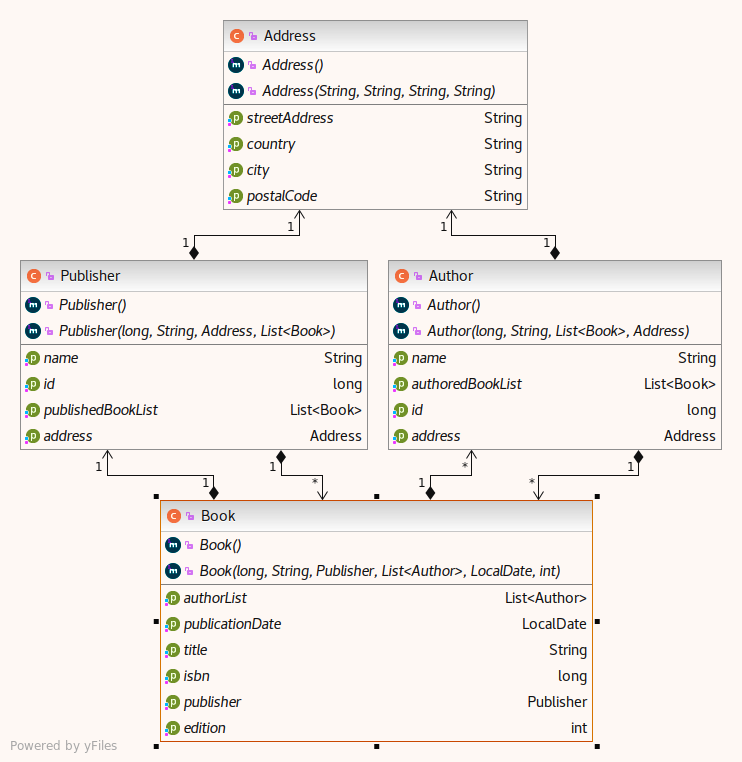
\includegraphics[width=12cm]{ajmt_uml.png}\\
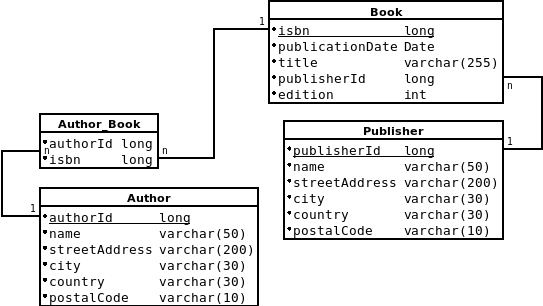
\includegraphics[width=10cm]{ajmt_schema.png}\\
\end{questions}

\bibliographystyle{plainnat}
\bibliography{ajexam1}

\end{document}